% !TeX root = ../main.tex

\section{Introduzione}
% cos'è devops, la filosofia devops, no silos, ecc
A causa della continua evoluzione delle tecnologie e all'aumento della concorrenza le aziende hanno bisogno di realizzare prodotti sempre più velocemente mantenendo e possibilmente aumentando la qualità~\cite{krief2019learning}. In risposta a questo problema è nata una vera e propria cultura, chiamata DevOps, la quale definisce sia un modo di pensare che una metodologia di lavoro fortemente basata sulla collaborazione tra i diversi team.

Fornisce infatti un insieme di pratiche al fine di ridurre le barriere tra il team di sviluppo (Dev) e il team operativo (Ops). Da un lato gli sviluppatori vogliono innovare e rilasciare software velocemente, mentre dall'altro lato l'obiettivo è quello di garantire la stabilità e la qualità dei sistemi. Oltre alla collaborazione tra i diversi team esistono altri principi alla base della cultura DevOps:
\begin{itemize}
    \item \textbf{Automazione} - L'intervento umano deve essere ridotto il più possibile al fine di ridurre gli errori e le tempistiche. In questo modo vengono rimossi tutti i compiti ripetitivi che sarebbero stati a carico dello sviluppatore facendogli risparmiare tempo.
    \item \textbf{Monitoraggio} - Deve essere possibile analizzare in ogni momento lo stato dei processi che compongono il sistema con lo scopo di reagire, prevenire e prevedere le situazioni critiche ma anche fornire feedback allo sviluppatore per aumentare la qualità del prodotto.
\end{itemize}

\section{Tecniche di automazione e vantaggi}
Ogni azienda ha i propri vincoli, requisiti e metodi i quali la rendono unica e per questo motivo non esiste un unico modo di utilizzo del DevOps. Esistono invece diverse tecniche che rispettano i principi DevOps e che possono essere applicate e adattate ad ogni azienda al fine di aumentare la qualità del software prodotto e diminuire il time-to-market (TTM)~\cite{devis2016effective}.

I principali benefici nell'adozione della cultura DevOps sono~\cite{krief2019learning}:
\begin{itemize}
    \item Migliore comunicazione e collaborazione all'interno dei team con un impatto umano e sociale a livello aziendale.
    \item Tempi di consegna in produzione minori che comportano un aumento delle performance e della soddisfazione dell'utente finale.
    \item Risparmio di tempo e risorse dovuti dall'utilizzo di un ciclo di sviluppo iterativo e tecniche di automazione.
\end{itemize}

I team che intendono adottare le tecniche DevOps nel proprio processo di sviluppo devono seguire metodologie Agile con fasi iterative che permettono maggiore qualità delle funzionalità e feedback rapidi da parte dell'utente. Le principali pratiche che vengono adottate sono: (\textit{i}) Continuous Integration, (\textit{ii}) Continuous Delivery, (\textit{iii}) Continuous Deployment e (\textit{iv}) Continuous Monitoring.

\begin{figure}[H]
    \centering
    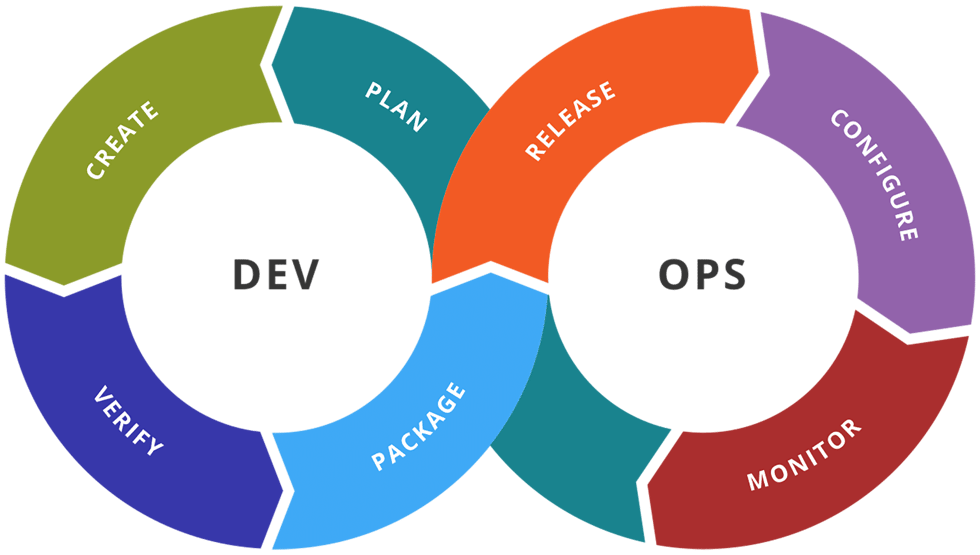
\includegraphics[width=0.6\textwidth]{img/Devops-toolchain.png}
    \caption{Fasi del ciclo di sviluppo software con tecniche DevOps.}
\end{figure}

\subsection{Continuous Integration}
\label{ci-sec}
Maggiore è la complessità di un progetto e maggiore è la necessità di integrare frequentemente e preventivamente i componenti software al fine di verificare che essi funzionino correttamente~\cite{duvall2007continuous}. Con Continuous Integration (CI) si intende una pratica di sviluppo software dove i membri di un team integrano frequentemente il loro lavoro e ogni integrazione è testata e verificata da un sistema automatico in grado di intercettare gli errori il più velocemente possibile\footnote{\href{https://martinfowler.com/articles/continuousIntegration.html}{https://martinfowler.com/articles/continuousIntegration.html}}.

Con pipeline si intende una sequenza ordinata di elaborazioni che vengono applicate al codice sorgente in modo automatico. Solitamente una pipeline di CI prevede tre task:

\begin{itemize}
    \item \textbf{Build} - Il primo task consiste nella verifica della corretta compilazione del codice sorgente.
    \item \textbf{Test} - Successivamente si eseguono i task di testing, tipicamente riguardanti la logica applicativa (unit testing).
    \item \textbf{Package} - Lo scopo dell'ultimo task della pipeline di CI consiste nella verifica della corretta pacchettizzazione del codice. Deve essere possibile creare correttamente l'artefatto che verrà poi passato alle fasi successive di rilascio (delivery).
\end{itemize}

\begin{figure}[H]
    \centering
    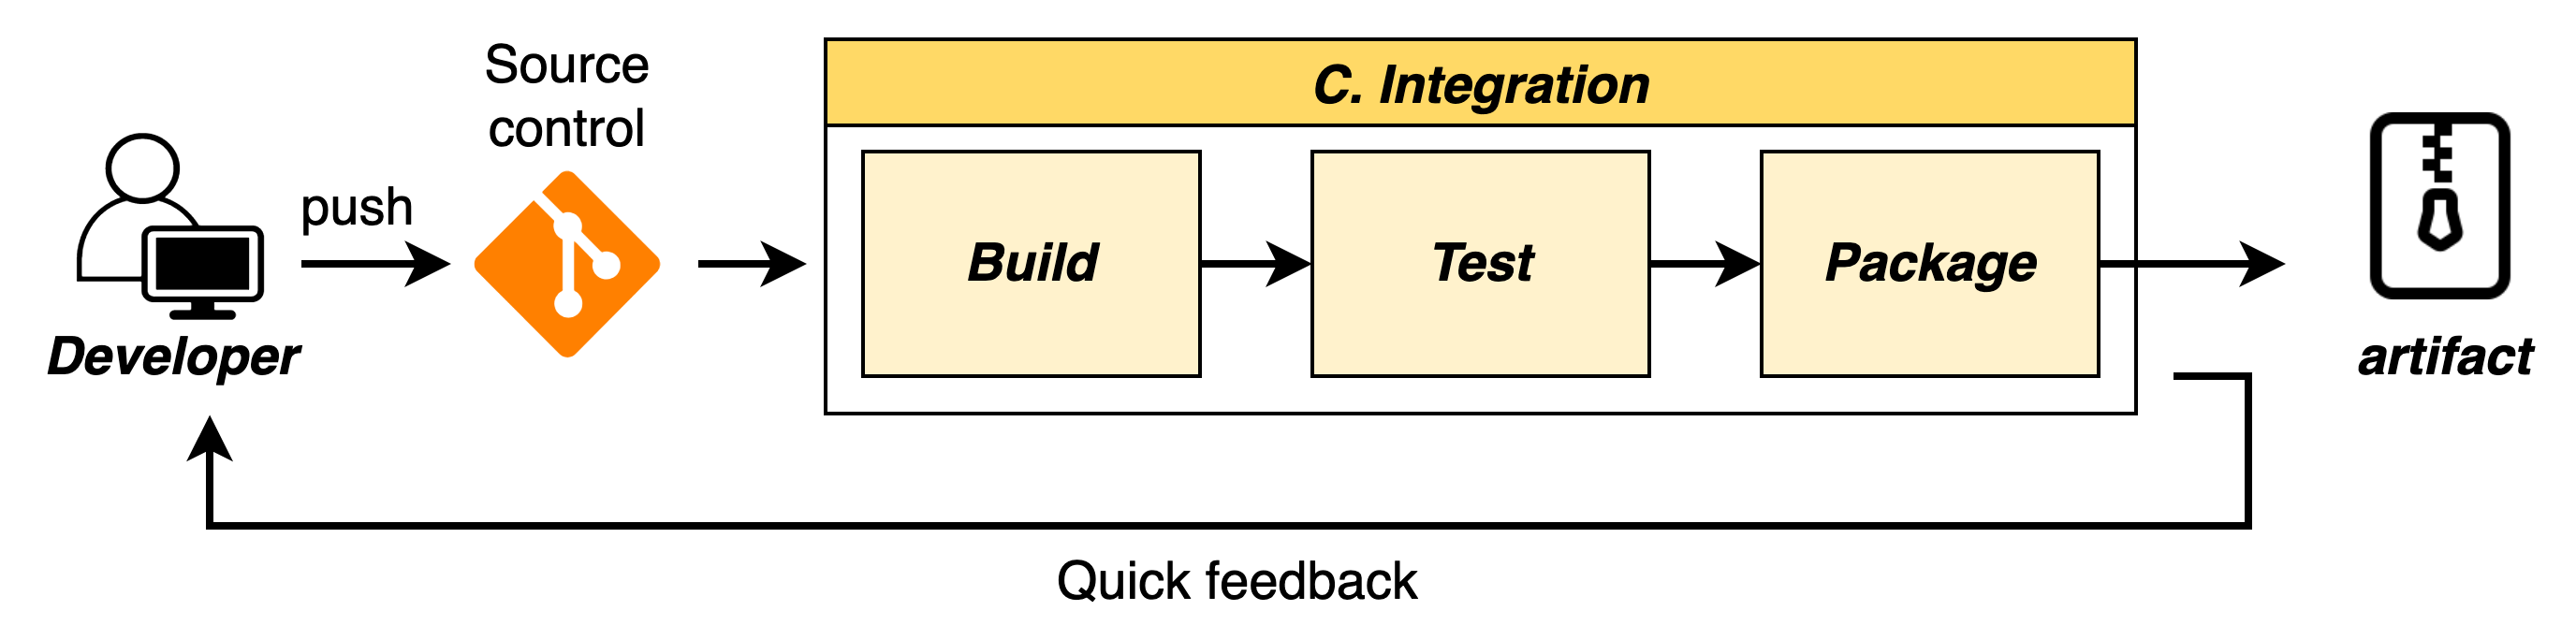
\includegraphics[width=0.9\textwidth]{img/ci-pipeline.png}
    \caption{Pipeline di Continuous Integration.}
    \label{ci-pipeline}
\end{figure}

Ogni sviluppatore lavora effettuando piccole modifiche al codice (commit) che possono essere facilmente sistemate in caso di errori: maggiore è la modifica applicata al codice e maggiore è il rischio di problemi. Grazie ai sistemi di versionamento del codice (VCS\footnote{Version Control System}) e alle funzionalità che forniscono come branch, commit, pull request e code review gli sviluppatori possono collaborare sul codice. Unendo le funzionalità dei VCS con le funzionalità di altri sistemi appositi per l'automazione di task, come GitLab CI, GitHub Actions e Travis CI è possibile adottare efficacemente le tecniche di CI nel processo di sviluppo. Tali strumenti a supporto dei sistemi di automazione sono descritti in modo dettagliato nella sezione \ref{devops-tools-sec} di questo capitolo.

\subsection{Continuous Delivery}
\label{cd-sec}
Quando la fase di CI termina con successo si continua con la fase successiva di rilascio automatico del codice. Con Continuous Delivery (CD) si intende una pratica di sviluppo dove il software viene sviluppato in una maniera tale da poter essere installato nell'ambiente di produzione in qualsiasi momento\footnote{\href{https://martinfowler.com/bliki/ContinuousDelivery.html}{https://martinfowler.com/bliki/ContinuousDelivery.html}}. Questo significa che gli stessi concetti di (\textit{i}) piccole modifiche e (\textit{molto frequentemente}) applicati alla fase di integrazione vengono applicati anche alla fase di rilascio.

Il compito principale della fase di CD è quello di prendere il software impacchettato nell'ultimo task della fase di CI (package) e renderlo disponibile alla fase successiva di installazione (deployment) tramite la pubblicazione su appositi sistemi chiamati package manager.

\begin{figure}[H]
    \centering
    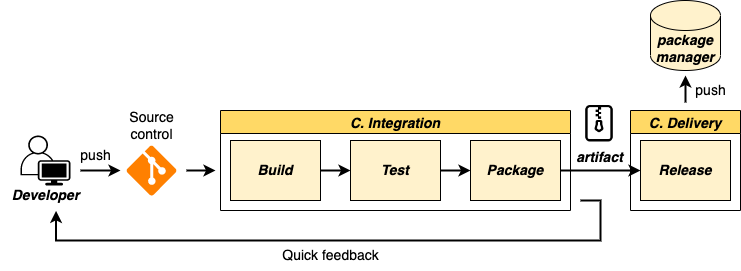
\includegraphics[width=1\textwidth]{img/cd-pipeline.png}
    \caption{Pipeline di Continuous Delivery.}
    \label{cd-pipeline}
\end{figure}

I package manager devono fornire lo spazio necessario alla archiviazione dei pacchetti creati durante la fase di CI e pubblicati durante la fase di CD ma devono anche supportare altre funzionalità come versionamento dei pacchetti, diverse tipologie di pacchetto e autenticazione per il caricamento/scaricamento dei pacchetti in caso di package manager privati. Alcuni esempi di package manager sono Nexus, Maven Central Repository e NPM.

E' fondamentale che il pacchetto pubblicato sul package manager sia dato come output dalla fase di CI in modo da garantire che il codice sorgente ha passato con successo tutti i task di controllo e verifica. Lo stesso pacchetto sarà poi utilizzato nella fase successiva per l'installazione in un ambiente d'esecuzione. 

\subsection{Continuous Deployment}
In base alla natura del software che si sviluppa il processo potrebbe terminare con la fase di delivery, come ad esempio nel caso di librerie e applicazioni mobile oppure continuare con l'installazione del prodotto in un ambiente di esecuzione, come nel caso di applicazioni web e microservizi. 

Nel caso in cui sia necessaria l'installazione del prodotto in un ambiente, la fase di deployment recupera il pacchetto pubblicato in fase di delivery e lo installa. Infatti, non può esistere continuous deployment senza continuous delivery, ma non è vero il contrario.

Con Continuous Deployment si intende quindi una estensione della continuous delivery con un processo che automatizza l'intera pipeline dal momento in cui lo sviluppatore modifica il codice alla installazione di quella modifica nell'ambiente di staging o produzione~\cite{krief2019learning}.

\begin{figure}[H]
    \centering
    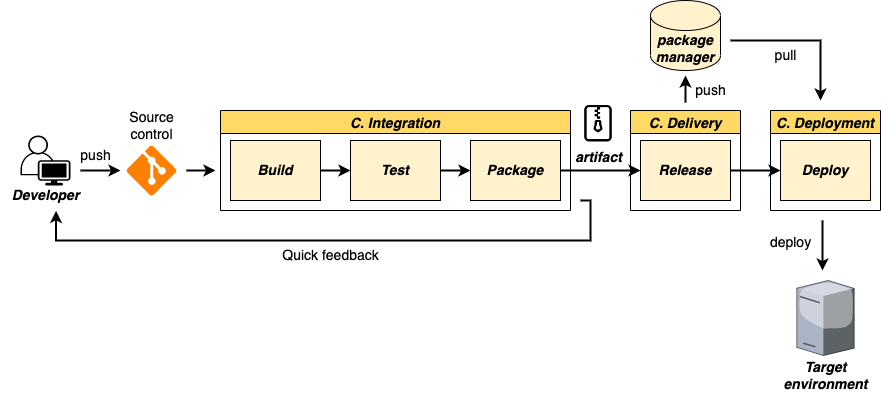
\includegraphics[width=1\textwidth]{img/cdeploy-pipeline.png}
    \caption{Pipeline di Continuous Delivery.}
    \label{cdeploy-pipeline}
\end{figure}

\subsection{Continuous Monitoring}
Poter raccogliere dati dal sistema per poterlo analizzare è uno dei punti chiave del DevOps poiché permette di migliorare sia il prodotto che il processo: garantisce integrità, prestazioni e affidabilità in ogni fase del ciclo di vita del software.

\begin{figure}[H]
    \centering
    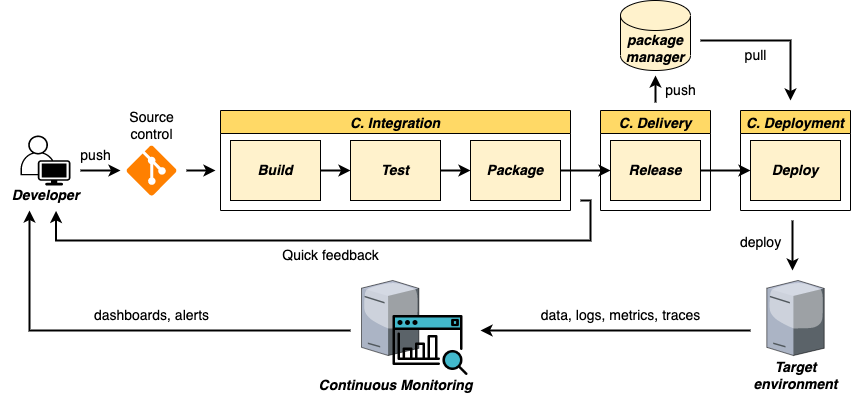
\includegraphics[width=1\textwidth]{img/ci-monitoring.png}
    \caption{Funzionamento tipico di un sistema di Continuous Monitoring.}
    \label{ci-monitoring}
\end{figure}

Anche la fase di monitoring deve essere continua e automatica ma a differenza della CI/CD, le pratiche di monitoraggio eseguono task che riguardano tutto il processo indipendentemente dal lavoro svolto dallo sviluppatore. Ad esempio:

\begin{itemize}
    \item raccolta di metriche riguardanti il processo di sviluppo (commit effettuate, merge request chiuse e approvate, issues, pipeline fallite, ...),
    \item raccolta di metriche riguardanti il software rilasciato (numero di download effettuati, recensioni, ...),
    \item raccolta di metriche riguardanti l'ambiente d'esecuzione del software installato (log, metriche, traces),
    \item centralizzazione di tutti i dati raccolti,
    \item invio di notifiche (alerting) al raggiungimento di una certa soglia da parte di una specifica metrica,
    \item creazione di dashboard per la visualizzazione grafica.
\end{itemize}

Lo scopo principale della pratica di continuous monitoring è ridurre il più possibile il tempo che intercorre tra il momento in cui un difetto è introdotto nel codice o nel processo, intercettato e risolto.

Le stesse pratiche si possono adottare per il monitoraggio dell'utente con l'obiettivo di raccogliere dati sul suo comportamento per migliorare l'esperienza utente, fare analisi di mercato o creare raccomandazioni. Tipicamente ci si riferisce a questa pratica con il termine analytics.

\subsection{Continuous Inspection}
Tipicamente vengono definiti a livello aziendale degli standard di qualità e di sicurezza
che devono essere rispettati da ogni team di sviluppo per qualsiasi prodotto software. La
definizione di linee guida sullo stile di programmazione o sul livello di severity accettato sono esempi di standard di qualità. La pratica di analizzare automaticamente e molto frequentemente il codice al fine di validare il rispetto degli standard di qualità e sicurezza è chiamata Continuous
Inspection.

L’obiettivo è quello di ottenere un feedback sullo stato del codice, sullo stato
del processo e sulla presenza di problemi di sicurezza al fine di pianificare interventi
risolutivi nel minor tempo possibile. Come nel caso del monitoraggio esiste un sistema terzo a supporto dei task necessari e in grado di fornire feedback allo sviluppatore. I principali task di analisi che compongono la fase di ispezione continua sono:

\begin{itemize}
    \item \textbf{Static Application Security Testing} (SAST) - Analisi white-box della applicazione al fine di individuare vulnerabilità, code smell e bug ma anche di verificare il rispetto di un certo livello di qualità.
    \item \textbf{Software Composition Analysis} (SCA) - Analisi delle dipendenze di progetto con lo scopo di individuare vulnerabilità pubbliche (CVE\footnote{Common Vulnerability and Exposure}) associate ad esse.
\end{itemize}

In entrambe le tipologie di analisi è fondamentale ottenere come risultato un report della scansione, in grado di descrivere in modo dettagliato eventuali entità individuate dalla fase di analisi. I report vengono prodotti tipicamente sia in formati human-readable (es. pagina HTML) che machine-readable (es. JSON, XML) per poter essere utilizzati da applicazioni terze come ad esempio sistemi centralizzati per la consultazione di report eterogenei chiamati Vulnerability Management System.

\begin{figure}[H]
    \centering
    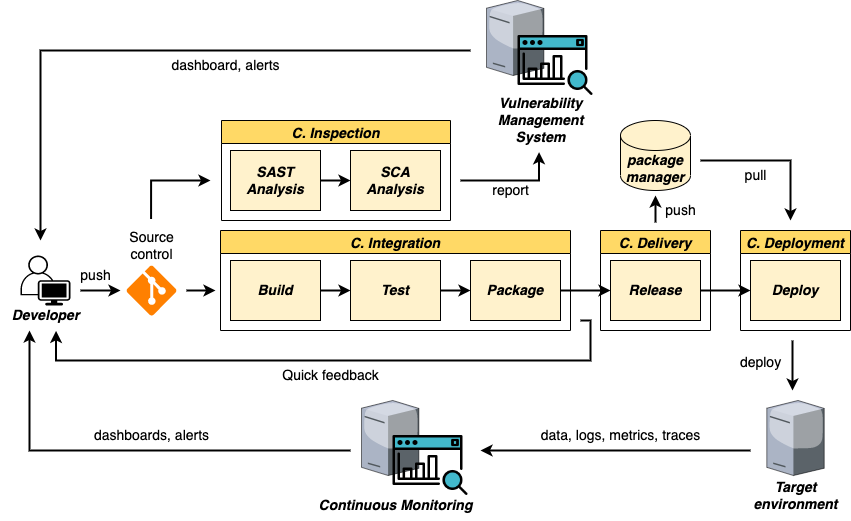
\includegraphics[width=1\textwidth]{img/cinspection-pipeline.png}
    \caption{Funzionamento tipico di un sistema di Continuous Inspection.}
    \label{ci-inspection-pipeline}
\end{figure}

\section{Strumenti}
\label{devops-tools-sec}
Per poter mettere in pratica le tecniche di CI/CD in modo da adottarle efficacemente nel processo di sviluppo è necessaria una infrastruttura complessa composta da tanti servizi e strumenti. Data la grande complessità soprattutto nella gestione, manutenzione e integrazione di tutti questi componenti spesso si fa uso di una o piu piattaforme cloud in modo da avere a disposizione un sistema in grado di fornire i seguenti strumenti fondamentali:
\begin{itemize}
    \item \textbf{Source control version} - Strumento per il versionamento del codice e tracciamento delle modifiche che permette la collaborazione tra i componenti di un team. Con l'avvento delle metodologie agile e della cultura DevOps, l'uso di un VCS nei processi è diventato obbligatorio.
    \item \textbf{Package Manager} - Strumento per l'archiviazione e la condivisione del software sviluppato sotto forma di pacchetti, come descritto nella sezione \ref{cd-sec}.
    \item \textbf{CI Server} - Strumento in grado di eseguire elaborazioni in modo automatico su un server remoto e restituire il risultato. Rappresenta il motore di tutta la automazione a supporto delle tecniche CI/CD.
\end{itemize}

\subsection{Pipeline as Code}
Nella sezione \ref{ci-sec} il concetto di pipeline è stato definito come una sequenza ordinata di elaborazioni che vengono applicate al codice sorgente in modo automatico. In realtà una pipeline di CI/CD è suddivisa in più passi, detti stage, i quali contengono una o più elaborazioni, dette job.

Lo strumento adottato da quasi tutte le principali piattaforme per la definizione degli stage e dei job che compongono una pipeline e quindi per istruire un CI Server all'esecuzione effettiva dei task è chiamato Pipeline as Code. Questo metodo permette di descrivere il processo di una pipeline in un file testuale, tipicamente in formato YAML, che si trova nello stesso repository in cui risiede il codice sorgente.

Il seguente listato contiene la definizione di una pipeline descritta utilizzando la sintassi per la piattaforma specifica GitLab. In questo caso la pipeline è composta da due stage (\textit{build} e \textit{deploy}), ognuno dei quali contiene a sua volta un job. Il cuore del job, ovvero le istruzioni bash che il CI Server deve eseguire sono definite tramite la keyword \textit{script}.

\begin{listing}[H]
    \inputminted{yaml}{code/3-pipelineexample}
    \caption{Pipeline d'esempio per la piattaforma GitLab.}
\end{listing}

I vantaggi derivanti dall'utilizzo del meccanismo Pipeline as Code sono:
\begin{itemize}
    \item versionamento dei file che descrivono le pipeline di CI/CD in modo da tracciare anche le modifiche che vengono apportate al processo automatizzato,
    \item utilizzo di metodologie simili a quelle utilizzate nello sviluppo software (ereditarietà, incapsulamento, riuso, ...),
    \item i file che descrivono il processo sono accessibile a tutto il team ed è possibile collaborare alla sua modifica in modo identico allo sviluppo software.
\end{itemize}

\subsection{Runners}
L'architettura di un CI Server deve essere costruita in modo robusto e scalabile per poter supportare efficacemente le tecniche CI/CD. Basta un team con un numero minimo di sviluppatori e un numero minimo di progetti ai quali sono applicate le tecniche CI/CD e la metodologia di sviluppo agile per comprendere l'enorme quantità di lavoro a cui un CI Server può essere sottoposto.

Ogni evento che si verifica sulla piattaforma in cui è mantenuto il codice sorgente viene intercettato dal CI Server: se nel file che descrive la pipeline è definito un job in associazione a quello specifico evento, il CI Server invia tutte le informazioni utili per l'esecuzione del job ad un altro componente software chiamato runner e rimane in attesa del risultato. 

\begin{figure}[H]
    \centering
    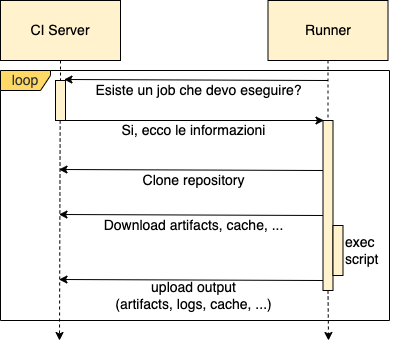
\includegraphics[width=0.6\textwidth]{img/ciserver-runner.png}
    \caption{Diagramma di sequenza interazione CI Server-Runner}
    \label{ci-server-runner}
\end{figure}

Il runner consiste in un componente architetturale della infrastruttura che necessita di un ambiente di esecuzione e per svolgere il suo compito consuma delle risorse. In base a chi lo gestisce il runner può essere:

\begin{itemize}
    \item \textbf{Managed} - Funzionalità fornita as-a-Service dalla piattaforma che si utilizza. In base al piano di licenza sottoscritto con la piattaforma l'utilizzo dei runner è soggetto a limiti che riguardano tipicamente i minuti di utilizzo e lo spazio di archiviazione. Il vantaggio di questa modalità è che non è richiesto alcuno sforzo nella configurazione e manutenzione del runner e nessuna spesa per l'ambiente di esecuzione.
    \item \textbf{Self-Hosted} - Il componente è gestito dall'utilizzatore in tutti i suoi aspetti ma non è soggetto ad alcun tipo di vincolo in termini di risorse utilizzate.
\end{itemize}